%%%%%%%%%%%%%%%%%%%%%%%%%%%%%%%%%%%%%%%%%
% Jacobs Landscape Poster
% LaTeX Template
% Version 1.0 (29/03/13)
%
% Created by:
% Computational Physics and Biophysics Group, Jacobs University
% https://teamwork.jacobs-university.de:8443/confluence/display/CoPandBiG/LaTeX+Poster
% 
% Further modified by:
% Nathaniel Johnston (nathaniel@njohnston.ca)
%
% This template has been downloaded from:
% http://www.LaTeXTemplates.com
%
% License:
% CC BY-NC-SA 3.0 (http://creativecommons.org/licenses/by-nc-sa/3.0/)
%
%%%%%%%%%%%%%%%%%%%%%%%%%%%%%%%%%%%%%%%%%

%----------------------------------------------------------------------------------------
%	PACKAGES AND OTHER DOCUMENT CONFIGURATIONS
%----------------------------------------------------------------------------------------

\documentclass[final]{beamer}

\usepackage[scale=1.24]{beamerposter} % Use the beamerposter package for laying out the poster

\usetheme{confposter} % Use the confposter theme supplied with this template

\setbeamercolor{block title}{fg=black,bg=white} % Colors of the block titles

\setbeamercolor{block body}{fg=black,bg=white} % Colors of the body of blocks
\setbeamercolor{block alerted title}{fg=white,bg=dblue!70} % Colors of the highlighted block titles
\setbeamercolor{block alerted body}{fg=black,bg=dblue!10} % Colors of the body of highlighted blocks
% Many more colors are available for use in beamerthemeconfposter.sty

%-----------------------------------------------------------
% Define the column widths and overall poster size
% To set effective sepwid, onecolwid and twocolwid values, first choose how many columns you want and how much separation you want between columns
% In this template, the separation width chosen is 0.024 of the paper width and a 4-column layout
% onecolwid should therefore be (1-(# of columns+1)*sepwid)/# of columns e.g. (1-(4+1)*0.024)/4 = 0.22
% Set twocolwid to be (2*onecolwid)+sepwid = 0.464
% Set threecolwid to be (3*onecolwid)+2*sepwid = 0.708

\newlength{\sepwid}
\newlength{\onecolwid}
\newlength{\twocolwid}
\newlength{\threecolwid}
\setlength{\paperwidth}{48in} % A0 width: 46.8in
\setlength{\paperheight}{36in} % A0 height: 33.1in
\setlength{\sepwid}{0.024\paperwidth} % Separation width (white space) between columns
\setlength{\onecolwid}{0.22\paperwidth} % Width of one column
\setlength{\twocolwid}{0.464\paperwidth} % Width of two columns
\setlength{\threecolwid}{0.708\paperwidth} % Width of three columns
\setlength{\topmargin}{-0.5in} % Reduce the top margin size
%-----------------------------------------------------------

\usepackage{graphicx}  % Required for including images

\usepackage{booktabs} % Top and bottom rules for tables
\usepackage[utf8]{inputenc} % allow utf-8 input
\usepackage[T1]{fontenc}    % use 8-bit T1 fonts
\usepackage{url}            % simple URL typesetting
\usepackage{booktabs}       % professional-quality tables
\usepackage{amsfonts}       % blackboard math symbols
\usepackage{nicefrac}       % compact symbols for 1/2, etc.
\usepackage{microtype}      % microtypography

\usepackage{amsmath,graphicx}
\usepackage{bm}
\usepackage{url}
\usepackage{amsmath}
\usepackage{amsthm}
\usepackage{graphicx}
%\usepackage{subcaption}
\usepackage{algorithm2e}
\usepackage{pbox}
\usepackage{multirow}

\usepackage{booktabs, multicol, multirow}
\usepackage{dirtree}
\usepackage{booktabs}
\usepackage{graphicx} 
\usepackage{amsmath}
\usepackage{booktabs, multicol, multirow}
\usepackage{pbox}
\usepackage{algorithm2e}
\usepackage[export]{adjustbox}
\renewcommand\DTstyle{}

\DeclareMathOperator{\argmax}{argmax}
\DeclareMathOperator{\argmin}{argmin}

\newcounter{savedenum}
\newcommand*{\saveenum}{\setcounter{savedenum}{\theenumi}}
\newcommand*{\resume}{\setcounter{enumi}{\thesavedenum}}

%----------------------------------------------------------------------------------------
%	TITLE SECTION 
%----------------------------------------------------------------------------------------

\title{Invariant Representations for Noisy Speech Recognition} % Poster title

\author{Dmitriy Serdyuk${}^{12}$, Kartik Audhkhasi${}^2$, Phil\'emon Brakel${}^1$,
    Bhuvana Ramabhadran${}^2$, Samuel Thomas${}^2$, \\
    Yoshua Bengio${}^{1 \dagger}$}

    \institute{${}^1$ MILA, Universit\'{e} de Montr\'{e}al, ${}^2$ IBM Watson, ${}^\dagger$ CIFAR Fellow} % Institution(s)

%----------------------------------------------------------------------------------------

\begin{document}
\addtobeamertemplate{headline}{} 
{
\begin{tikzpicture}[remember picture,overlay] 
\node [shift={(-13 cm,-7cm)}] at (current page.north east)
% \node [shift={(-10 cm,-5cm)}] at (current page.north west)
{
\includegraphics[height=7cm]{ibmpos_blue}}; 
%\node [shift={(-42 cm,-11cm)}] at (current page.north)
%{\includegraphics[height=7cm]{UdeM_CMJK.eps}}; 
\node [shift={(-49 cm,-6cm)}] at (current page.north)
% \node [shift={(-10 cm,-5cm)}] at (current page.north west)
{\includegraphics[height=9cm]{MILA_2C.eps}}; 
\end{tikzpicture} 
}

\addtobeamertemplate{block end}{}{\vspace*{2ex}} % White space under blocks
\addtobeamertemplate{block alerted end}{}{\vspace*{2ex}} % White space under highlighted (alert) blocks

\setlength{\belowcaptionskip}{2ex} % White space under figures
\setlength\belowdisplayshortskip{2ex} % White space under equations

\begin{frame}[t] % The whole poster is enclosed in one beamer frame

\begin{columns}[t] % The whole poster consists of three major columns, the second of which is split into two columns twice - the t option aligns each column's content to the top

\begin{column}{\sepwid}\end{column} % Empty spacer column

\begin{column}{\onecolwid} % The first column

%----------------------------------------------------------------------------------------
%	OBJECTIVES
%----------------------------------------------------------------------------------------

\begin{block}{Introduction}
    \begin{itemize}
        \item 
            \textcolor{dblue}{Robustness} to the acoustic variability arising from environmental, speaker, channel, 
    and recording 
    conditions is a challenge in modern day 
    neural network-based ASR systems, especially when all types of variability are 
    not seen during training. 
    
        \item We attempt to address this problem by encouraging the 
            neural network acoustic model to learn \textcolor{dblue}{invariant} feature representations.
        
        \item We use ideas from recent research on image generation using
            \textcolor{dblue}{generative adversarial networks} and domain adaptation ideas extending
    adversarial gradient-based training.  
        \item We evaluate the proposed 
    architecture on the Aurora-4 task, a popular benchmark for
    noise robust ASR. 
    \end{itemize}

\end{block}


%----------------------------------------------------------------------------------------
%	INTRODUCTION
%----------------------------------------------------------------------------------------

\begin{block}{Generative Adversarial Networks}
    \begin{itemize}
        \item Two networks: the generator and the discriminator.
        \item The generator network $G$ has an
    input of randomly-generated feature vectors and is asked to produce a sample, e.g. an image, 
    similar to the images in the training set. 
    
        \item The discriminator network $D$
    can either receive a generated image from the generator $G$ or an image
    from the training set. Its task is to distinguish
    between the ``fake'' generated image and the ``real'' image taken from the dataset~\cite{goodfellow2014generative}:
    \begin{align*}
        \min_G \max_D V(D, G) = & \mathbb{E}_{\bm{x} \sim p_{\text{data}}(\bm{x})}[\log D(\bm{x})] + \\
            & \mathbb{E}_{\bm{z} \sim p_{\bm{z}}(\bm{z})}[\log (1 - D(G(\bm{z})))].
    \end{align*}

    \end{itemize}


    \begin{block}{Domain Adaptation with Reverse Gradient}
        \begin{itemize}
            \item \cite{ganin2014unsupervised} proposes $Y$-shaped network: the image is fed to the
            encoder network ($E$) which produces a hidden representation $h$. 
            
            \item This representation $h$ is input to two separate networks: a domain classifier network ($D$) and 
            a target classifier network ($R$). 
            
            \item The goal of training is to learn the hidden 
            representation that is invariant to the domain labels and performs well on the target classification 
            task. 
            
            \item Similar to the GAN objective, which forces the generation distribution be close to the data distribution,
            the \emph{gradient reverse method} makes domain distributions similar to each other.
        \end{itemize}
        
    \end{block}
\end{block}

\end{column} % End of the first column

\begin{column}{\sepwid}\end{column} % Empty spacer column

\begin{column}{\twocolwid}

    \begin{columns}[t]

        \begin{column}{\onecolwid} % The second column
            \begin{block}{{\Large Invariant Representation Network}}
                \begin{itemize}
                    \item The model consists of three neural networks. 
                    \item The encoder $E$ produces
                        the intermediate representation $h$ which used in the recognizer $R$ and 
                        in the domain discriminator $D$. 
                    \item The hidden representation $h$ is trained to improve
                        the recognition and minimize the domain discriminator performance. 
                    \item The domain discriminator
                        is a classifier trained to maximize its accuracy on the noise type
                        classification task.
                \end{itemize}
                \begin{equation*}
                    L = L_1(\hat{y}, y; \theta_R, \theta_E) + 
                    \alpha L_2(\hat{d}, d; \theta_D) -
                    \beta L_3(\hat{d}, d; \theta_E)
                \end{equation*}

                \begin{figure}
                    \centering
                    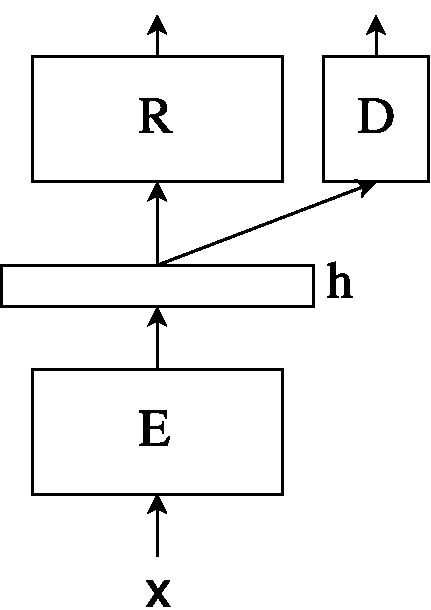
\includegraphics[width=0.9\linewidth]{model.pdf}
                \end{figure}

                \begin{itemize}
                    \item The model is a DNN-HMM system with a feed-forward neural network trained to predict the 
                        CD HMM state (2000 classes).
                    \item Input: 40-dimensional Mel-filterbank features with their deltas and 
                        delta-deltas spliced over $\pm$5 frames (total dimension is 1320).
                    \item Baseline: 6-layer DNN with 2048 rectified linear units at every layer.
                    \item The right branch that predicts the domain (noise condition). This branch is discarded 
                        in the testing phase. 
                    \item The noise condition is the domain label. We are merging all noise types into one label
                        and clean as the other label.
                    \item The invariance term is
                        \begin{equation*}
                            L_3 = d\log(1 - \hat{d}) + (1-d)\log(\hat{d}),
                        \end{equation*}
                        where $d$ is the domain label and $\hat{d}$ is the network prediction.
                \end{itemize}
            \end{block}

        \end{column} % end of second column

        \begin{column}{\sepwid}\end{column} % Empty spacer column

        \begin{column}{\onecolwid} % The third column
            \begin{block}{\Large Dataset}
                \begin{itemize}
                    \item Aurora-4 is based on the Wall Street Journal corpus (WSJ0). 
                    \item It contains noises of 
                        6 categories which was added to clean data. Every clean and noisy utterance is 
                        filtered to simulate the frequency characteristics. 
                    \item The training data: 
                        \begin{itemize}
                            \item One microphone: Sennheiser.
                            \item 4400 clean utterances.
                            \item 446 utterances for each of 6 noise condition.
                            \item Total of 2676 noisy utterances.
                        \end{itemize}
                    \item The testing set:
                        \begin{itemize}
                            \item Two microphones.
                            \item 330 utterances for each condition, each microphone.
                        \end{itemize}
                \end{itemize}
            \end{block}

            \begin{block}{{\Large Experiments on Aurora-4}}
                \begin{itemize}
                    \item We performed 6 experiments with different set of seen noises. 
                    \item The networks are trained
                on clean data, with each noise condition added one-by-one in the following order: airport, babble, car, 
                restaurant, street, and train:
                    \begin{enumerate}
                        \item clean + airport
                        \item clean + airport + babble
                        \item \ldots
                    \end{enumerate}
                \end{itemize}

                \begin{figure}
                    \centering
                    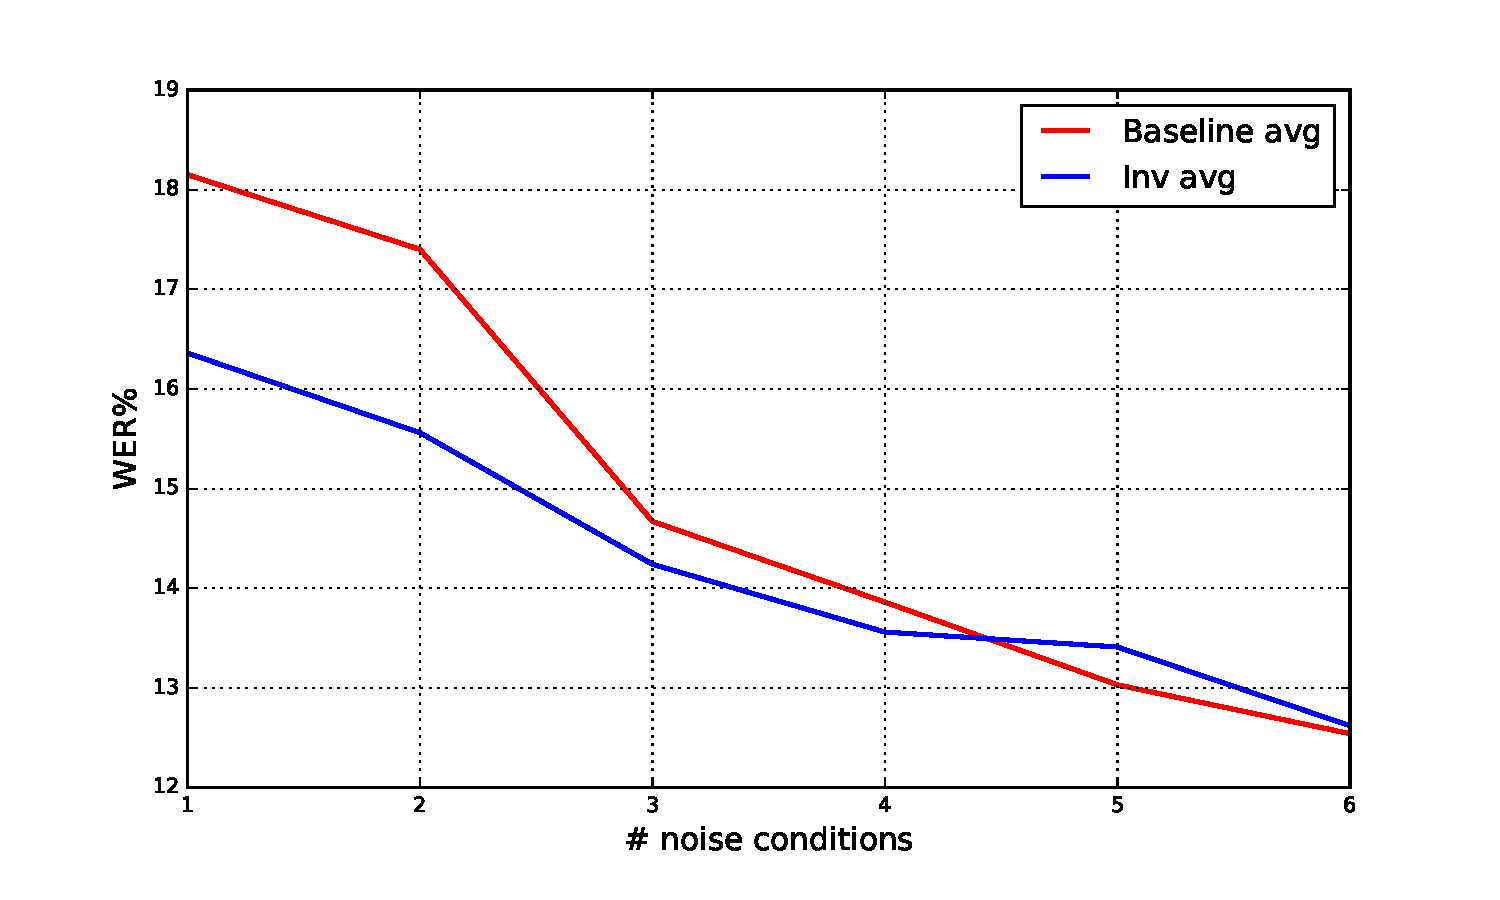
\includegraphics[width=\linewidth]{wer_avg.pdf}
                \end{figure}
                Average performance of the baseline multi-condition and invariance model varying with the 
                number of noise conditions used for training. 
                \begin{figure}
                    \centering
                    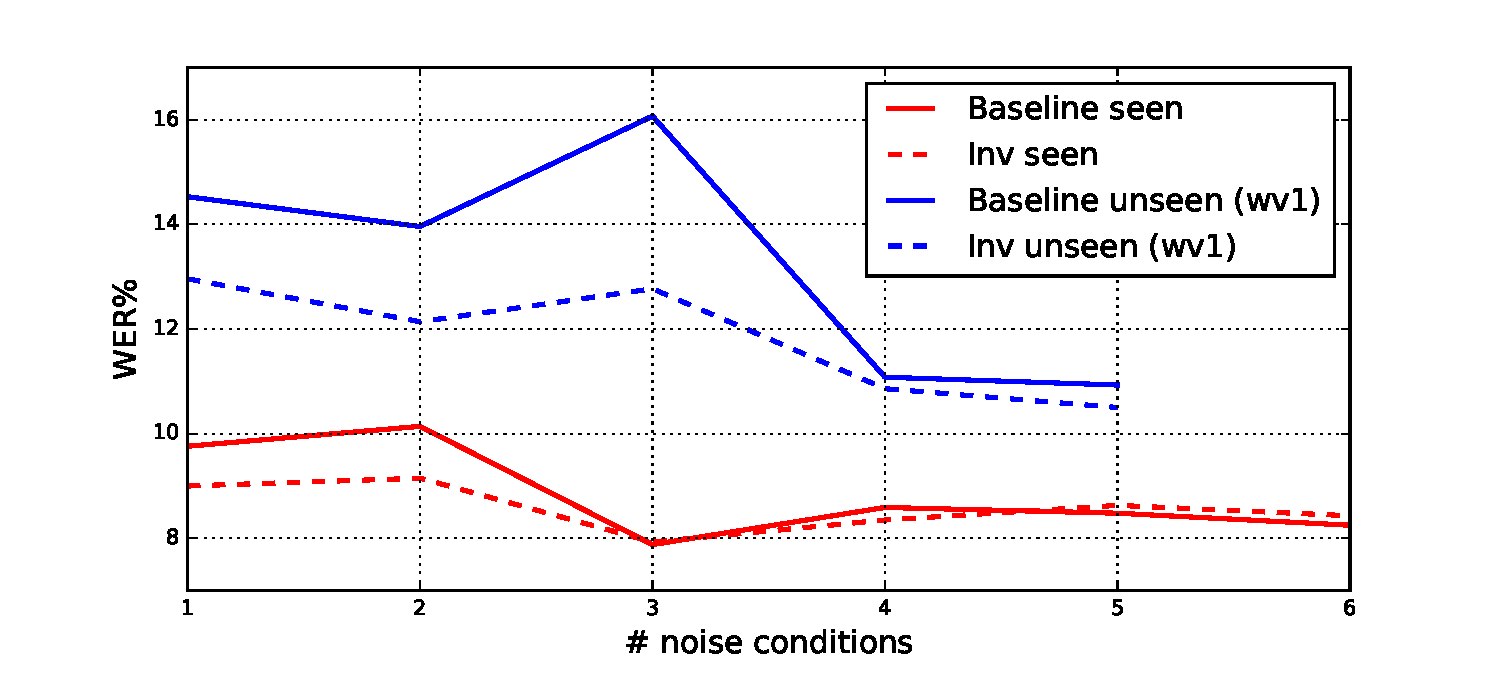
\includegraphics[width=\linewidth]{wer_seen_unseen.pdf}
                \end{figure}
                Average performance on seen versus 
                unseen noise conditions.
                Testing was performed on all wv1 conditions (Sennheiser microphone).
            \end{block}
        \end{column} % end of third column
    \end{columns}
\end{column}

\begin{column}{\sepwid}\end{column} % Empty spacer column
\begin{column}{\onecolwid} % the fourth column
\begin{block}{Results}

    Average word error rate (WER\%) on Aurora-4 dataset on all test conditions,
        including seen and unseen noise and unseen microphone. First column
        is the number of noise conditions used for the training. The last row is a 
        preliminary experiment with layer-wise pre-training close to state-of-the-art
        model and a corresponding invariance training starting with a pretrained model.
\begin{table}
    \centering
    \label{tab:results}
    \begin{tabular}{r|cc||cc|cc|cc|cc}
        Noise       &Inv&BL&  \multicolumn{2}{c|}{A} & \multicolumn{2}{c|}{B} & \multicolumn{2}{c|}{C} & \multicolumn{2}{c}{D}\\
        cond  & & &  Inv & BL & Inv & BL & Inv & BL & Inv & BL\\
    \hline
    1           &16.36        &18.14 &6.54&7.57    &12.71& 14.09   & 11.45&   13.10    & 22.47 &   24.80    \\
    2           &15.56        &17.39 &5.90&  6.58 &   11.69   &13.28   &11.12   &13.51   &21.79   &23.96 \\
    3           &14.24        &14.67 &5.45 & 5.08&    10.76&   12.44&   9.75&    9.84 &   19.93&   19.30\\
    4           &13.61        &13.84 & 5.08 &5.29    &9.73    &9.97    &9.49    &9.56    &19.49   &19.90\\         
    5           &13.41        &13.02 & 5.12 &5.34    &9.52    &9.42    &9.55    &8.67    &19.33   &18.65\\         
    6           &12.62        &12.60 & 4.80 &4.61    &9.04    &8.86    &8.76    &8.59    &18.16   &18.21\\
    \hline\hline
    6*          &11.85        &11.99 &4.52    &4.76    &8.76    &8.76    &7.79    &8.57    &16.84&    16.99
    \end{tabular}
\end{table}
\end{block}

\begin{block}{Conclusions}
    \begin{itemize}
        \item We show that invariance training helps the ASR system to generalize better to unseen noise 
            conditions and improves word error rate when a small number of noise types are seen during 
            training. 

        \item Related work~\cite{yusuke2016adversarial} investigates a similar approach for domain 
            adaptation to noise types and the SNR levels on an in-house dataset based on WSJ.
        
        \item Our experiments show that in contrast to the image recognition task, in speech recognition, the 
    gradient of the $L_3$ term is unreliable and noisy. 
    
        \item Future research includes enhancements to the domain adaptation network while exploring 
            alternative network architectures and invariance-promoting loss functions.
    \end{itemize}
\end{block}
%----------------------------------------------------------------------------------------
%	REFERENCES
%----------------------------------------------------------------------------------
\begin{block}{Important References}
    \bibliographystyle{amsalpha}
    \bibliography{refs.bib}
\end{block}
%----------------------------------------------------------------------------------------
%	ACKNOWLEDGEMENTS
%----------------------------------------------------------------------------------------

\setbeamercolor{block title}{fg=red,bg=white} % Change the block title color

%----------------------------------------------------------------------------------------
%	CONTACT INFORMATION
%----------------------------------------------------------------------------------------

%----------------------------------------------------------------------------------------

\end{column} % End of the third column

\end{columns} % End of all the columns in the poster

\end{frame} % End of the enclosing frame

\end{document}
